\section{Experiment}	\label{sec:experiments}

	\subsection{Basic SIP Analysis}
		The Session Initiation Protocol (SIP) is an application layer control protocol for establishing, changing and terminating multimedia sessions, where the sessions can be IP telephony, multimedia sessions or multimedia conferences. SIP is the core protocol of many IP-based PBX applications, including Asterisk.
		
		To demonstrate the main components of the SIP communication, a simplified scenario is implemented, as shown in Figure  \hyperref[fig:topo]{Figure \ref{fig:topo}}. Two softphone applications are running on the same computer, and an IP-based PBX application (Asterisk), running on a Raspberry Pi 4, is serving as the PBX server.
		
		\begin{figure}[htbp]
			\centerline{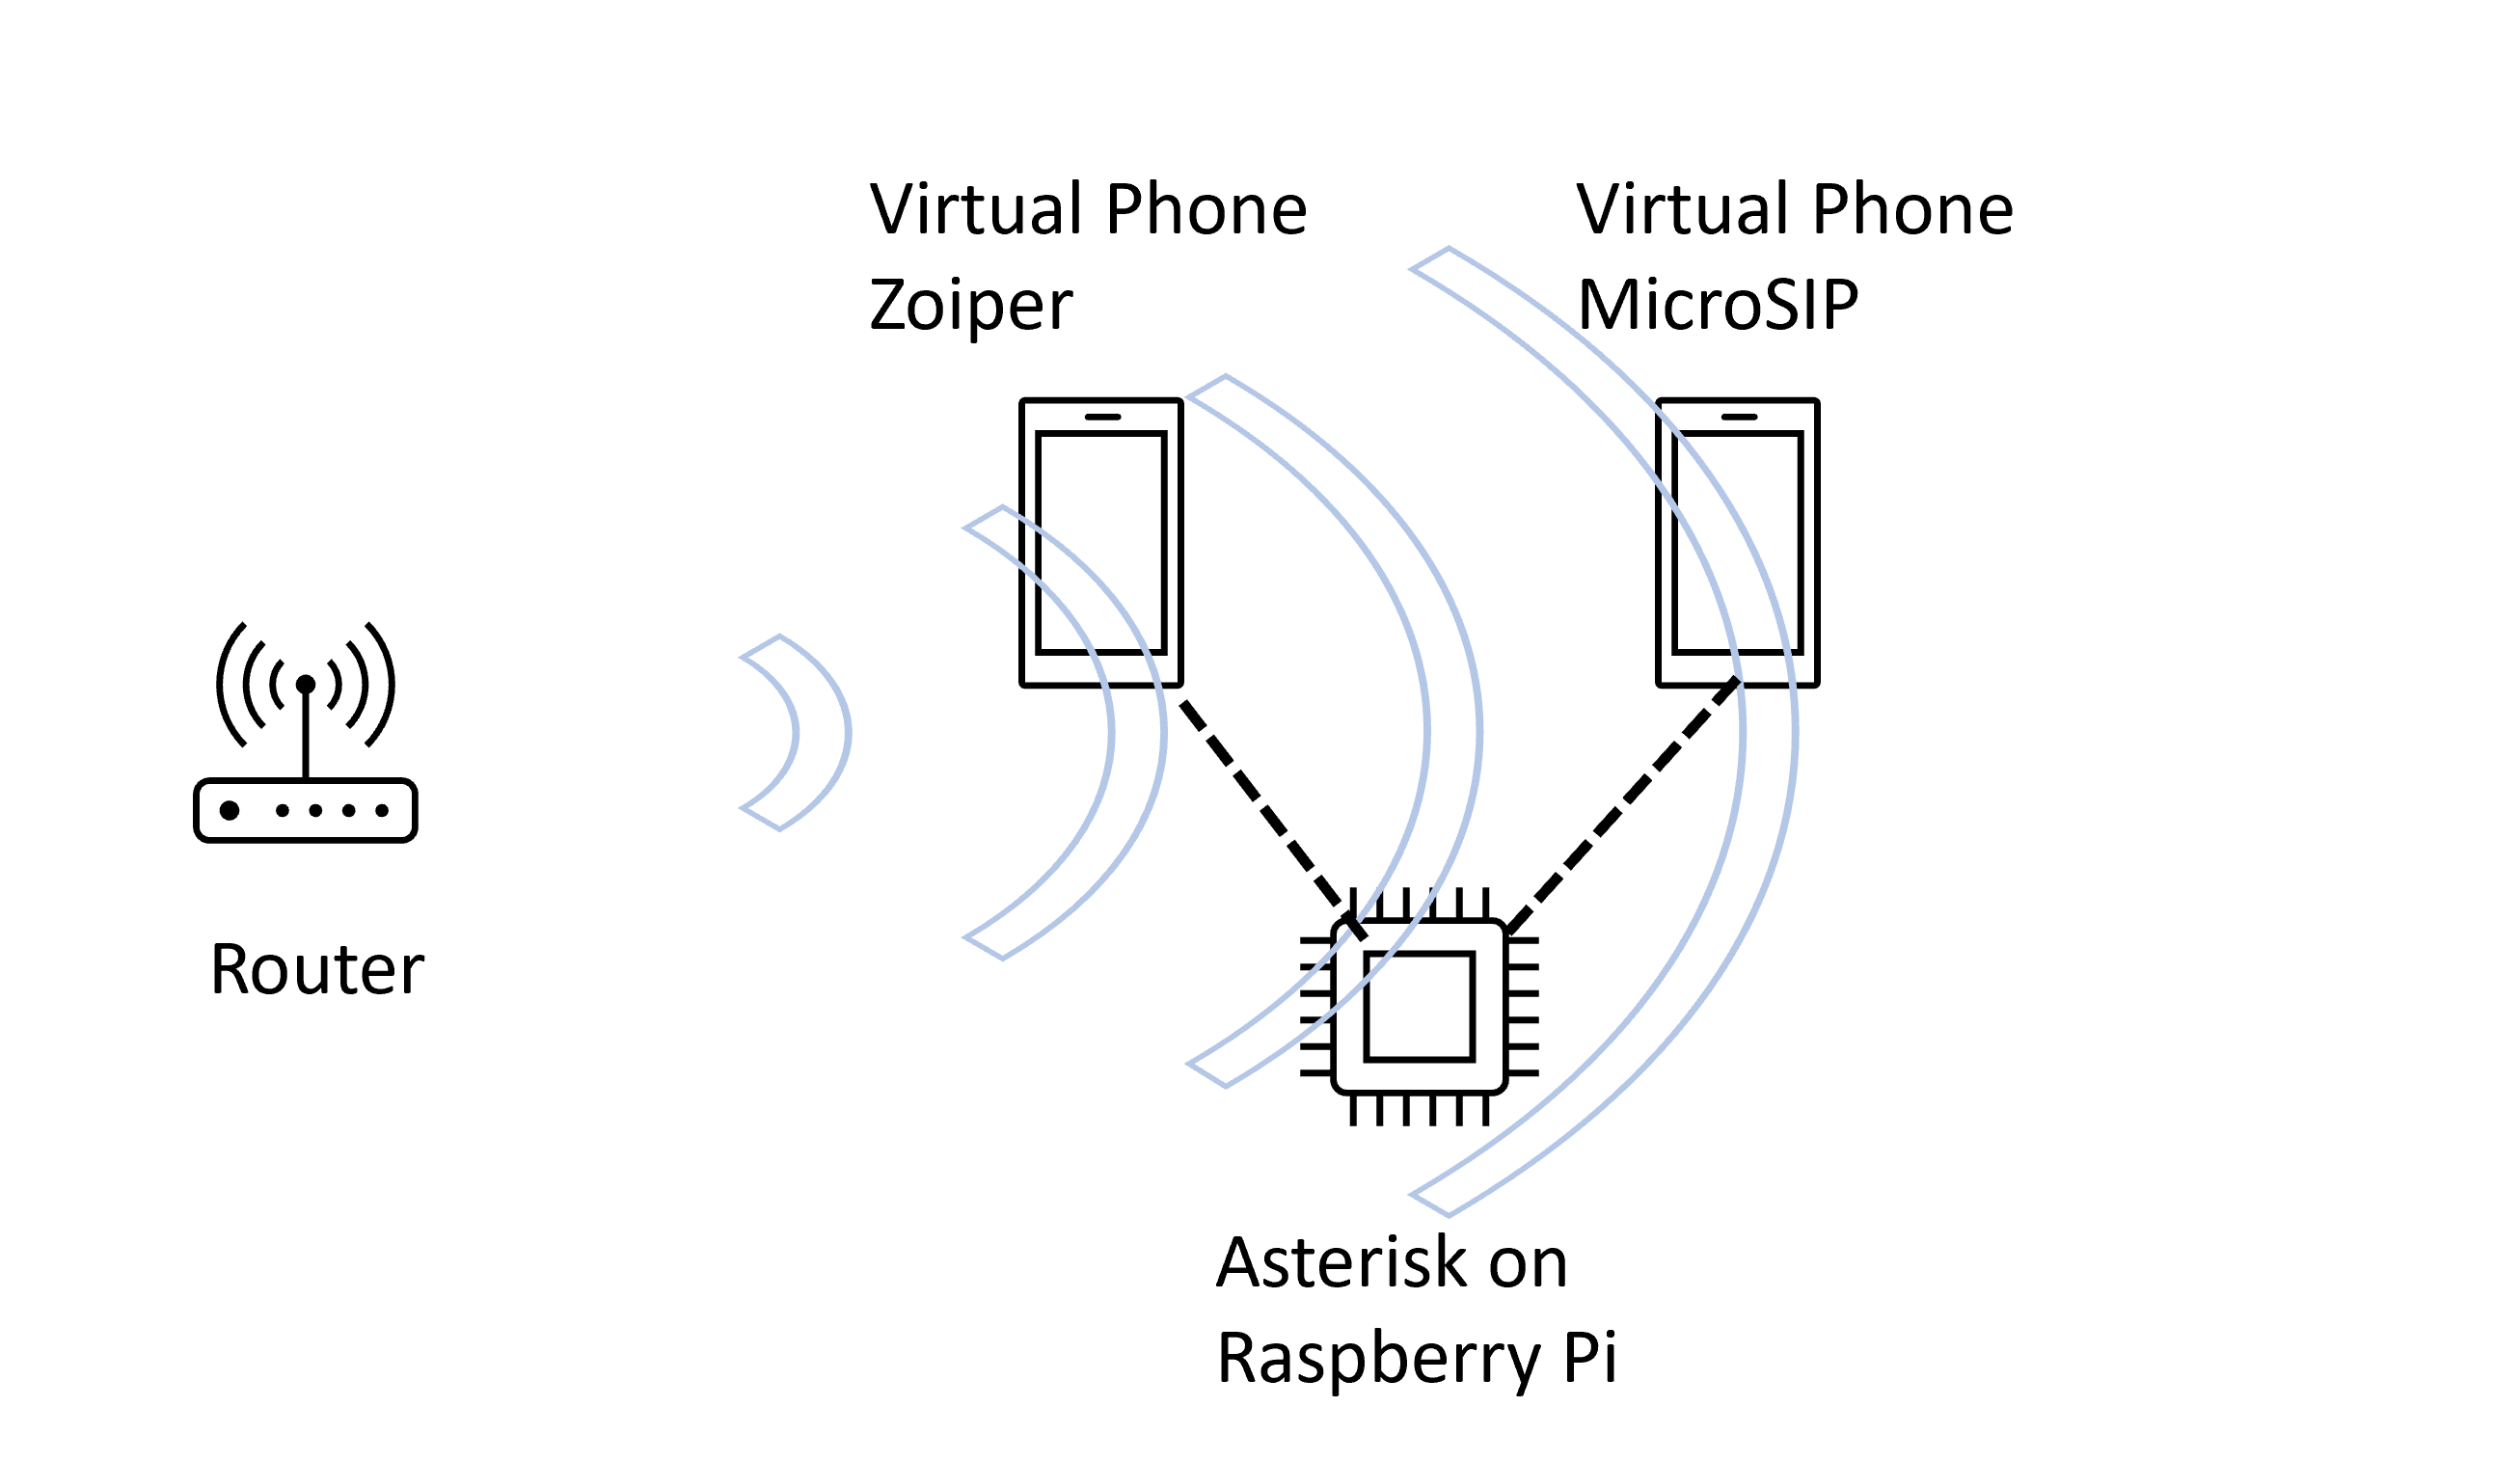
\includegraphics[width=8cm]{Images/experiment/exp1.png}}
			\caption{Simplified Scenario}
			\label{fig:topo}
		\end{figure}
		
		The SIP process starts with registration. All SIP terminals as User Agents should register with the registration server to inform their location, session capability, and other information.
		
		Usually, when the SIP terminal (User Agent) is powered on or configured to perform a registration operation, a registration request message (REGISTER) is sent to the registration server, carrying all the information that needs to be registered. After receiving the registration request message, the registration server sends a response message to the terminal to inform it that the request message has been received. If the registration is successful, it will send a "200 OK" message to the terminal. However, the most common response is a "401 Unauthorized" message because authorization is required in most of the implantations for security purposes. 
		
		To trace and see all types of packets tramissions, author used Wireshark open-souce software. \hyperref[fig:packet-trace]{Figure \ref{fig:packet-trace}} is a flow sequence of the one single call from Zoiper5 user (IP: 192.168.60.106:63771) to MicroSIP user (IP:192.168.60.106:53493). In this, senario their are actual two connections, first from Zoiper5 user to Asterisk (shown in left-side of Figure \ref{fig:packet-trace}) and second Asterisk to MicroSIP (shown in right-side of Figure \ref{fig:packet-trace}).
	
		The SIP protocol adopts the Client-Server pattern, in which the calls are established between User Agents through the proxy server.
				
		\begin{figure}[htbp]
			\begin{minipage}{0.24\textwidth}
				\begin{flushleft}
					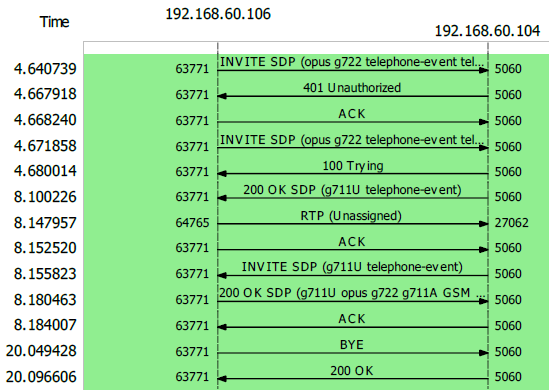
\includegraphics[height=100pt,width=\textwidth]{Images/experiment/a1.png}
%%					\caption{Zoiper to Asterisk}
				\end{flushleft}
			\end{minipage}
			\begin{minipage}{0.24\textwidth}
				\begin{flushright}
					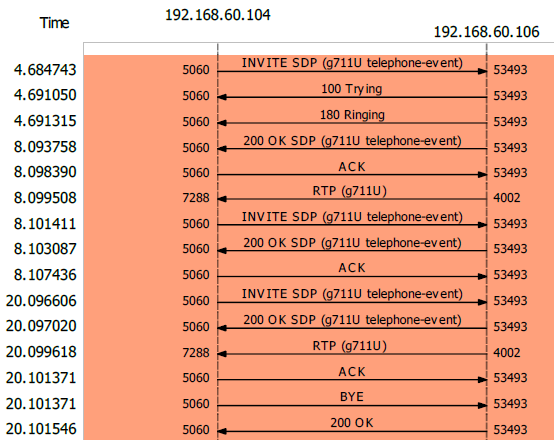
\includegraphics[height=100pt,width=\textwidth]{Images/experiment/a2.png}
%					\caption{Zoiper to MicroSIP}
				\end{flushright}
			\end{minipage}
			\caption{SIP packet trasmission from Zoiper to Asterisk(left-side), Asterisk to MicroSIP (right-side)}
			\label{fig:packet-trace}
		\end{figure}
				
